\section{Original Model}

The model of the sailboat come from~\cite{Melin2016} a modified version of the model in~\cite{LeBars2013}.



\begin{figure}[H]
\centering
\psscalebox{0.45 0.45} % Change this value to rescale the drawing.
{
% \usepackage[usenames,dvipsnames]{pstricks}
% \usepackage{epsfig}
% \usepackage{pst-grad} % For gradients
% \usepackage{pst-plot} % For axes
% \usepackage[space]{grffile} % For spaces in paths
% \usepackage{etoolbox} % For spaces in paths
% \makeatletter % For spaces in paths
% \patchcmd\Gread@eps{\@inputcheck#1 }{\@inputcheck"#1"\relax}{}{}
% \makeatother
% % User Packages:
% \usepackage{amsmath}
% \usepackage{amsfonts}
% \usepackage{amssymb}
% \usepackage{algorithm}
% \usepackage{algorithmic}
\psscalebox{1.0 1.0} % Change this value to rescale the drawing.
{
\begin{pspicture}(0,-6.3229065)(27.976694,6.3229065)
\definecolor{colour6}{rgb}{0.627451,0.627451,0.627451}
\definecolor{colour7}{rgb}{0.40392157,0.3882353,0.3882353}
\pspolygon[linecolor=black, linewidth=0.04, fillstyle=solid,fillcolor=black](4.2265778,0.6801973)(4.2265778,0.6687973)(4.1737776,0.6687973)(4.1737776,0.6801973)
\pspolygon[linecolor=black, linewidth=0.04, fillstyle=solid,fillcolor=black](4.2265778,0.6801973)(4.2265778,0.6687973)(4.1737776,0.6687973)(4.1737776,0.6801973)
\psline[linecolor=black, linewidth=0.02](4.494638,0.92061454)(4.494638,-5.747811)
\psline[linecolor=black, linewidth=0.02](4.5202856,0.92916393)(0.6303709,0.92916393)
\psline[linecolor=black, linewidth=0.04, arrowsize=0.05291667cm 2.0,arrowlength=1.4,arrowinset=0.0]{->}(0.65601873,-5.755437)(12.642086,-5.755437)
\psline[linecolor=black, linewidth=0.04, arrowsize=0.05291667cm 2.0,arrowlength=1.4,arrowinset=0.0]{->}(0.63892037,-5.755437)(0.63892037,5.409901)
\psline[linecolor=colour6, linewidth=0.03, linestyle=dashed, dash=0.17638889cm 0.10583334cm](0.65783095,-5.7774105)(6.7124696,4.760216)
\psline[linecolor=black, linewidth=0.020657333](1.7846738,-0.7115013)(4.5205197,-2.0897024)
\psline[linecolor=black, linewidth=0.02](5.956275,3.439544)(4.5137773,-2.090031)
\psline[linecolor=black, linewidth=0.02](5.956275,3.446615)(1.7843451,-0.72531486)
\rput[bl](4.325926,-6.3229065){{\huge $x$}}
\rput[bl](0.0,0.5215381){{\huge $y$}}
\psarc[linecolor=colour7, linewidth=0.03, linestyle=dashed, dash=0.17638889cm 0.10583334cm, dimen=inner, arrowsize=0.05291667cm 2.0,arrowlength=1.4,arrowinset=0.0]{->}(4.4962683,0.90230674){0.44}{19.308674}{310.4}
\rput[bl](4.44457,1.4879671){{\Large $w$}}
\psarc[linecolor=black, linewidth=0.04, linestyle=dashed, dash=0.17638889cm 0.10583334cm, dimen=outer, arrowsize=0.05291667cm 2.0,arrowlength=1.4,arrowinset=0.0]{->}(0.67470086,-5.742382){1.16}{0.0}{58.991932}
\rput[bl](1.8318518,-4.7999434){{\LARGE $\theta$}}
\rput[bl](0.8096296,5.5111675){{\huge North }}
\rput[bl](10.942963,-5.5110545){{\huge East}}
\rput[bl](16.698519,-5.103647){{\LARGE $\theta$}}
\rput[bl](23.935556,-3.555499){{\LARGE $\psi_{tw}$}}
\rput[bl](17.683704,1.4222788){{\LARGE $\psi_{aw}$}}
\psarc[linecolor=black, linewidth=0.03, linestyle=dashed, dash=0.17638889cm 0.10583334cm, dimen=outer, arrowsize=0.05291667cm 2.0,arrowlength=1.4,arrowinset=0.0]{->}(18.638119,-0.08968701){1.16}{60.0}{190.0}
\psarc[linecolor=black, linewidth=0.03, linestyle=dashed, dash=0.17638889cm 0.10583334cm, dimen=outer, arrowsize=0.05291667cm 2.0,arrowlength=1.4,arrowinset=0.0]{->}(23.642906,-5.004217){1.16}{0.0}{127.42864}
\rput[bl](21.683704,-2.086553){{\LARGE $a_{tw}$}}
\rput[bl](22.29624,5.598347){{\LARGE $v$}}
\rput[bl](13.711624,0.35219333){{\LARGE $-v$}}
\rput[bl](14.480855,-1.3093451){{\LARGE $a_{aw}$}}
\rput[bl](16.650085,2.5675778){{\LARGE $a_{tw}$}}
\psarc[linecolor=black, linewidth=0.04, linestyle=dashed, dash=0.17638889cm 0.10583334cm, dimen=outer, arrowsize=0.05291667cm 2.0,arrowlength=1.4,arrowinset=0.0]{->}(15.365983,-5.727294){1.16}{0.0}{58.991932}
\psline[linecolor=colour6, linewidth=0.03, linestyle=dashed, dash=0.17638889cm 0.10583334cm](23.691505,-5.0271945)(27.976694,-5.0271945)
\psline[linecolor=black, linewidth=0.03, arrowsize=0.05291667cm 2.0,arrowlength=1.4,arrowinset=0.0]{->}(23.6699,-5.027194)(21.300167,-2.0771163)
\psline[linecolor=black, linewidth=0.02](20.27553,2.7457647)(16.1036,-1.4261652)
\psline[linecolor=black, linewidth=0.02](20.27553,2.7386935)(18.833033,-2.7908812)
\psline[linecolor=black, linewidth=0.020657333](16.10393,-1.4123517)(18.839773,-2.7905526)
\psline[linecolor=colour6, linewidth=0.03, linestyle=dashed, dash=0.17638889cm 0.10583334cm](15.3684845,-5.779089)(20.284313,2.7476165)
\psline[linecolor=colour6, linewidth=0.03, linestyle=dashed, dash=0.17638889cm 0.10583334cm](15.36854,-5.755247)(27.354607,-5.755247)
\psline[linecolor=black, linewidth=0.02, arrowsize=0.05291667cm 2.0,arrowlength=1.4,arrowinset=0.0]{->}(18.5919,-0.11845798)(14.142602,-0.868068)
\psline[linecolor=black, linewidth=0.02, arrowsize=0.05291667cm 2.0,arrowlength=1.4,arrowinset=0.0]{<-}(14.094239,-0.868068)(16.270527,2.8799818)
\psline[linecolor=black, linewidth=0.02, arrowsize=0.05291667cm 2.0,arrowlength=1.4,arrowinset=0.0]{->}(20.187843,2.6260817)(22.36413,6.3741317)
\psline[linecolor=black, linewidth=0.02, arrowsize=0.05291667cm 2.0,arrowlength=1.4,arrowinset=0.0]{->}(18.640263,-0.09427698)(16.270525,2.855801)
\psline[linecolor=black, linewidth=0.03, arrowsize=0.05291667cm 2.0,arrowlength=1.4,arrowinset=0.0]{->}(11.099177,2.5849168)(12.309377,4.802627)
\psline[linecolor=black, linewidth=0.02](8.240868,-2.2198353)(8.265048,-4.444484)
\psline[linecolor=black, linewidth=0.02](9.348247,-0.36297163)(10.122038,-2.9261541)
\psline[linecolor=colour6, linewidth=0.03, linestyle=dashed, dash=0.17638889cm 0.10583334cm](7.2482057,-3.906535)(11.091619,2.5942028)
\psline[linecolor=black, linewidth=0.020657333](6.924077,-1.5593172)(9.659923,-2.9375184)
\psline[linecolor=black, linewidth=0.02](11.095678,2.591728)(9.65318,-2.937847)
\psline[linecolor=black, linewidth=0.02](11.095678,2.598799)(6.9237485,-1.5731308)
\psarc[linecolor=black, linewidth=0.018, linestyle=dashed, dash=0.17638889cm 0.10583334cm, dimen=outer, arrowsize=0.05291667cm 2.0,arrowlength=1.4,arrowinset=0.0]{->}(8.234815,-2.2332768){1.2222222}{240.0}{270.0}
\psarc[linecolor=black, linewidth=0.018, linestyle=dashed, dash=0.17638889cm 0.10583334cm, dimen=outer, arrowsize=0.05291667cm 2.0,arrowlength=1.4,arrowinset=0.0]{->}(9.346443,-0.3774628){1.2222222}{240.0}{287.0}
\rput[bl](7.5814815,-4.0621657){{\LARGE $\delta_r$}}
\rput[bl](8.994815,-2.3243878){{\LARGE $\delta_s$}}
\rput[bl](11.391396,4.5316806){{\LARGE $v$}}
\end{pspicture}
}


}
    \caption{Representation of the state vector variable and the inputs $\delta_s$ and $\delta_r$ and representation of the true wind and apparent wind.}
    \label{fig:drawing_boat_ink}
\end{figure}


\begin{equation}
\begin{bmatrix}
\dot{x}\\
\dot{y}\\
\dot{\theta}\\
\dot{v}\\
\dot{\omega}
\end{bmatrix}\  = \begin{bmatrix}
v \cos(\theta)+p_1 a_{tw} \cos(\psi_{tw})\\
v \sin(\theta)+p_1 a_{tw} \sin(\psi_{tw})\\
\omega\\
(g_s \sin(\delta_s)-g_r p_{11} \sin(\delta_r) - p_2 v^2)/p_9\\
(g_s(p_6-p_7\cos(\delta_s))-g_r p_8 \cos(\delta_r)-p_3 \omega v)/p_{10}
\end{bmatrix}
\end{equation}


The states boat is represented by different variables $x$ and $y$ for the position of the boat, a heading $\theta$ 
and an angular speed $\omega$.
The model is non-holonomic such as the boat will always go in the direction $\theta$ (minus the wind drift) therefore the speed $v$ is defined in the boat frame as for the input $[ \delta_s , \delta_r]$, where $\delta_r$ is the rudder angle and $\delta_s$ is the angle of the sail (which is proportional to the sheet length).


$g_s$ and $g_r$ are the force on the sail and on the rudder:
\begin{align}
g_s &= p_4 a_{aw} \sin(\delta_s - \psi_{aw})\\
g_r &= p_5 v^2 \sin(\delta_r)
\end{align}

The force on the sail depend on the apparent wind:

\begin{equation}
\bf{W}_{c,aw}= \begin{bmatrix}
a_{tw} \cos(\psi_{tw} -\theta) - v\\
a_{tw} \sin(\psi_{tw} -\theta)
\end{bmatrix}\
\end{equation}

\begin{equation}
\bf{W}_{p,aw}=\begin{bmatrix}
a_{aw}\\
\psi_{aw}
\end{bmatrix} = \begin{bmatrix}
\mid \bf{W}_{c,aw}\mid\\
\textnormal{angle}( \bf{W}_{c,aw})
\end{bmatrix}\
\end{equation}

$a_{tw}$ is the true wind speed and $\psi_{tw}$ its direction in the world frame
and $a_{aw}$ is the apparent wind speed on the boat and $\psi_{aw}$ the direction of the apparent wind in the boat frame.\\
\begin{minipage}{\linewidth}
\centering
\captionof{table}{Parameters correspondance} \label{tab:title2} 
\begin{center}
\begin{tabular}[t]{|c|l|l|}%{|m{0.10\linewidth}|m{0.3\linewidth}|m{0.1\linewidth}|}
\hline
 $p_1$ & drift coefficient & - \\ \hline
 $p_2$ & tangential friction & $kgs^{-1}$\\ \hline
 $p_3$ & angular friction & $kgm$ \\ \hline
 $p_4$ & sail lift & $kgs^{-1}$ \\ \hline
 $p_5$ & rudder lift & $kgs^{-1}$ \\ \hline
 $p_6$ & distance to sail & $m$ \\ \hline
 \end{tabular}
 \begin{tabular}[t]{|c|l|l|}%{|m{0.10\linewidth}|m{0.3\linewidth}|m{0.1\linewidth}|}
\hline
 $p_7$ & distance to mast & $m$ \\ \hline
 $p_8$ & distance to rudder & $m$ \\ \hline
 $p_9$ & mass of boat & $kg$ \\ \hline
 $p_{10}$ & moment of inertia & $kgm^2$ \\ \hline
 $p_{11}$ & rudder break coefficient & - \\ \hline
\end{tabular}
\end{center}
\end{minipage}
\bigskip

The goal of this model is to be simple, not to experience the real reaction of a sailboat but
to be able to implement a controller for this ship. This kind of reasoning has been successful in the past 
with this model and others (see~\cite{LeBars2013}~\cite{Melin2016}).

\section{Adding the cable force}

The design of this model originated from the model in this paper~\cite{Jaulin2015} and changed after that.
This model will separate the cable simulation and the sailboat. Having a cable on the boat, changes its dynamic 
and the model need to be updated to take into account the new forces applying on the boat.
\subsection{Modification of this model}
\paragraph*{Adding drifting}
~\\
%\vskip1mm
\hskip7mm 

Having a cable on the boat will make it not follow the normal path 
Here $\alpha_{c}$ is the direction of the force of the cable on the boat in the world frame and $g_c$ its norm.
$v_c$ represent the effect of the cable on the boat, it doesn't depend on the direction of boat when calculating its speed, and $\alpha_{v}$ is the direction of this drift. 


\begin{equation}
\begin{bmatrix}
\dot{x}\\
\dot{y}\\
\dot{\theta}\\
\dot{v}\\
\dot{v_{c,x}}\\
\dot{v_{c,y}}\\
\dot{\omega}
\end{bmatrix}\  = \begin{bmatrix}
v \cos(\theta)+v_{c,x}+p_1 a_{tw} \cos(\psi_{tw})\\
v \sin(\theta)+v_{c,y}+p_1 a_{tw} \sin(\psi_{tw})\\
\omega\\
(g_s \sin(\delta_s)-g_r p_{11} \sin(\delta_r)+ g_c \cos(\alpha_c-\theta) - p_2 v^2)/p_9\\
(-(p_2+p_{12} \sin^2(\alpha_v-\theta))(v_{c,x} \mid v_{c,x} \mid ) + g_c \sin(\alpha_{c} -\theta) \cos(\theta+\pi/2))/p_9\\
(-(p_2+p_{12} \sin^2(\alpha_v-\theta))(v_{c,y} \mid v_{c,y} \mid ) + g_c \sin(\alpha_{c} -\theta) \sin(\theta+\pi/2))/p_9\\
(g_s(p_6-p_7\cos(\delta_s))-g_r p_8 \cos(\delta_r)-p_3 \omega v)/p_{10}
\end{bmatrix}
\end{equation}

But the effect this drifting depend on the direction of the boat.
If the drift make the boat go in a orthogonal direction the friction of the boat will be more important than if it
drag the boat on the same direction therefore the computation of friction :

\begin{equation}
\textnormal{friction} = (p_2+p_{12} \sin^2(\alpha_v-\theta))
\end{equation}

When $\alpha_v = \theta \pmod{\pi}$ the boat goes in the same direction of the drift therefore the friction is equal to the tangential friction $p_2$. But when $\alpha_v -\theta =\pm \pi/2$ the friction created by the drift is orthogonal to the boat so the friction is at its maximum.

But the cable does not always make the boat drift, if the cable pull in the same direction of the boat, the force 
will directly impact the speed  $v$ of the boat (without making it drift). The effect of the cable is distributed between $\dot{v}$ and $\dot{v_c}$ depending on the difference $\alpha_c -\theta$.

\paragraph*{Changing Application point of the force from the cable}
~\\
\vskip1mm
\hskip7mm
 
The point of effect of the cable force may not be at the center of inertia of the boat therefore it will
have an effect on the angular acceleration. The angular acceleration formula is changed to the following  when
the cable is place on the median of the boat:
\begin{equation}
\dot{\omega} =
(g_s(p_6-p_7\cos(\delta_s))-g_r p_8 \cos(\delta_r)-p_3 \omega v -p_{13} g_c \sin(\alpha_c-\theta))/p_{10}
\end{equation}

With $-p_{13} g_c \sin(\alpha_c-\theta)$ being the effect of the cable on the angular acceleration.
This mean the cable will often have a breaking effect to the rotation of the boat.

\begin{figure}[H]
\centering
    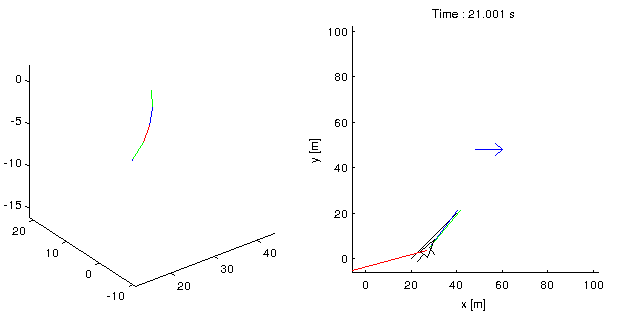
\includegraphics[scale=0.7,angle=0]{under_way_cable_no_delay.png}
    \caption{Simulation display representing first the cable, then the boat.}
    \label{fig:3wayBoat}
\end{figure}

In figure~\ref{fig:3wayBoat} is represented the cable \footnote{To see simulation : \href{https://www.youtube.com/watch?v=1nrbdikXr8A}{Simulation of a boat with a cable on it}},and the boat with in red the force of the cable on the boat and the blue arrow is the wind direction.

\subsection{Simulation Results}

The boat behave differently whereas it have a cable attached or not. The boat is slower and have a longer response time also.

\begin{figure}[H]
\centering
    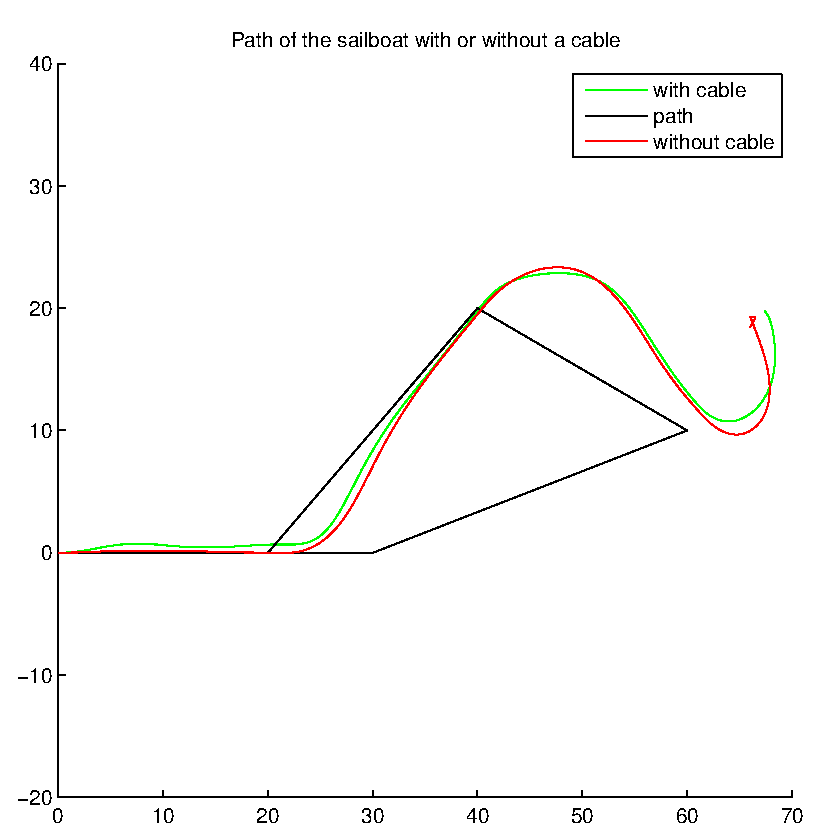
\includegraphics[scale=0.4,angle=0]{path_w_wtFig}
    \caption{Path taken by the boat with or without cable.}
    \label{fig:pathBoat}
\end{figure}

In figure~\ref{fig:pathBoat} the path of the boat with or without cable is represented, the boat is controlled each time by the algorithm from Le Bars and Jaulin 2013~\cite{LeBars2013}. The boat is less controllable in a straight
line, indeed the boat start at the position zero in the direction of the wind, the boat without cable follow very thoroughly the line but the boat with cable discard from the line.

The boat with cable looks more efficient when turning, but it would be because of the lesser speed.

